% !TEX program = xelatex

\documentclass{resume}
\usepackage{graphicx}
\usepackage{tabu}
\usepackage{multirow}
\usepackage{progressbar}
%\usepackage{zh_CN-Adobefonts_external} % Simplified Chinese Support using external fonts (./fonts/zh_CN-Adobe/)
%\usepackage{zh_CN-Adobefonts_internal} % Simplified Chinese Support using system fonts

\begin{document}
\pagenumbering{gobble} % suppress displaying page number

{
% change Large font here
\Large{
  \begin{tabu}{ c l r }
   \multirow{5}{1in}{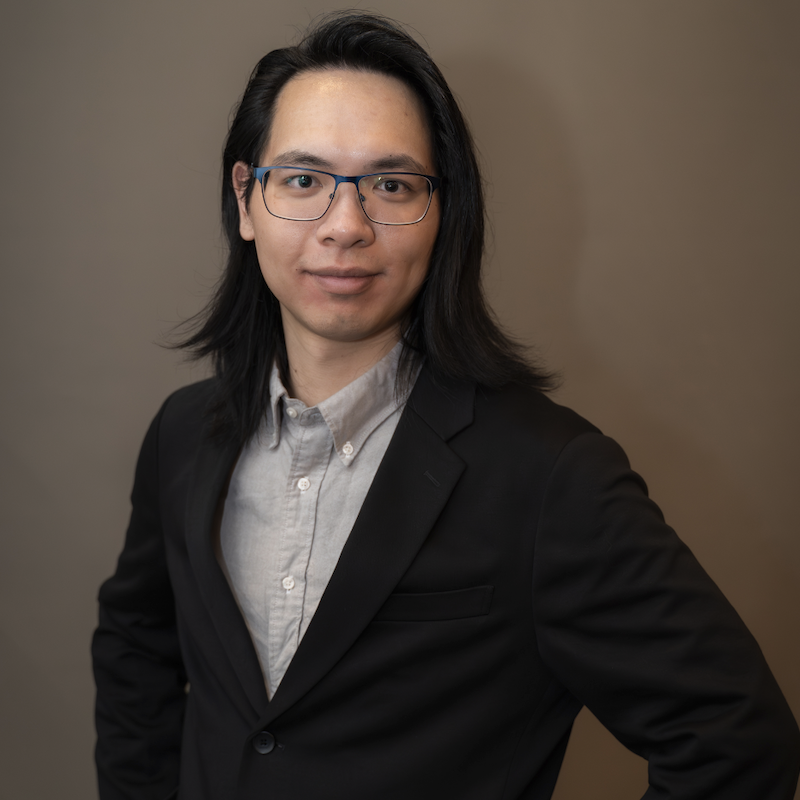
\includegraphics[width=0.88in]{avatar}} & \scshape{Roy Xu} & {Python~}\progressbar{0.4} \\
    & \email{section0.com@gmail.com} & {Flask~}\progressbar{0.3} \\
    & \phone{(+61) (0)431-332-881} & {Linux~}\progressbar{0.5} \\
    & \linkedin[realroyxu]{https://www.linkedin.com/in/realroyxu/}\\
    & \github[github.com/realroyxu]{https://github.com/realroyxu}
  \end{tabu}
}
}

\section{\faGraduationCap\ Education}
\datedsubsection{\textbf{University of Western Australia}, WA, Australia}{2023 -- Present}
\textit{Bachelor student} in Computer Science, expected Jun 2025
\datedsubsection{\textbf{Foshan University}, Foshan, China}{2020 -- 2022}
\textit{Bachelor student} in Computer Science

\section{\faUsers\ Experience}
\datedsubsection{\textbf{Backup Project}}{March. 2024 -- Present}
\role{Collaborte with UCC's Wheel group}{}
Brief introduction: Help setting up a backup solution (twin Dell R710) for UCC servers, 
\begin{itemize}
  \item Setup iDRAC, update old firmwares
  \item Testing hardwares, mainly the HBA cards
  \item Collecting opinions, help deciding the HDD models
\end{itemize}


\datedsubsection{\textbf{UCC Inc.} WA, Australia}{Feb. 2024 -- Present}
\role{Ordinary Committee Member}{}
Brief introduction: OCM of University Computer Club, https://ucc.asn.au/infobase/committee/2024/
\begin{itemize}
  \item Help running the club
  \item Some assistance in tech issues
\end{itemize}


\datedsubsection{\textbf{CITS3403 Project}}{May. 2024}
\role{SQL, Flask, Ajax/API}{University Unit Project, collaborated with Aifert Yet}
A Flask website for UWA unit CITS3403, https://github.com/realroyxu/CITS3403-MurderMystery
\begin{itemize}
  \item Database, Backend logic, Page design
  \item REST API for most operations
\end{itemize}

\datedsubsection{\textbf{Lambda Studio/Foshan University}}{Oct. 2020 -- May. 2022}
\role{Sysadmin assistance}
Brief introduction: System Ops for Foshan University's homepage and its supporting systems
\begin{itemize}
  \item Website CD with Gitlab and Jenkins
  \item Docker Swarm configuration and maintaining
  \item Setup and operating selfhosted Zabbix, goharbor, CTFD, and NSfocus security platform
  \item Daily system monitoring and incident responding/patching
\end{itemize}

% Reference Test
%\datedsubsection{\textbf{Paper Title\cite{zaharia2012resilient}}}{May. 2015}
%An xxx optimized for xxx\cite{verma2015large}
%\begin{itemize}
%  \item main contribution
%\end{itemize}

\section{\faCogs\ Skills}
\begin{itemize}[parsep=0.5ex]
  \item Programming Languages: Python > Java > C
  \item Platform: Linux
  \item Git, team collaboration
\end{itemize}

% \section{\faHeartO\ Honors and Awards}
% \datedline{\textit{\nth{1} Prize}, Award on xxx }{Jun. 2013}
% \datedline{Other awards}{2015}

\section{\faInfo\ Miscellaneous}
\begin{itemize}[parsep=0.5ex]
  \item GitHub: https://github.com/realroyxu
  \item Languages: English - Fluent, Mandarin - Native speaker
\end{itemize}

\section{\faFax\ Referee}
\datedsubsection{\textbf{Grace Fowler}}{}
\role{President of UCC}
\begin{itemize}
  \item Mail: fowleg20@gmail.com
  \item Phone: (+61) (0)475-622-858
\end{itemize}

%% Reference
%\newpage
%\bibliographystyle{IEEETran}
%\bibliography{mycite}
\end{document}
